\documentclass[a4paper,UTF8]{article}
\usepackage{ctex}
\usepackage[margin=1.25in]{geometry}
\usepackage{color}
\usepackage{graphicx}
\usepackage{amssymb}
\usepackage{amsmath}
\usepackage{amsthm}
\usepackage{bbm}
\usepackage{enumerate}
\usepackage{bm}
\usepackage{hyperref}
\usepackage{epsfig}
\usepackage{color}
\usepackage{tcolorbox}
\usepackage{mdframed}
\usepackage{lipsum}
\usepackage{mathtools}
\newmdtheoremenv{thm-box}{myThm}
\newmdtheoremenv{prop-box}{Proposition}
\newmdtheoremenv{def-box}{定义}
\newcommand{\norm}[1]{\left\lVert#1\right\rVert}

\setlength{\evensidemargin}{.25in}
\setlength{\textwidth}{6in}
\setlength{\topmargin}{-0.5in}
\setlength{\topmargin}{-0.5in}
% \setlength{\textheight}{9.5in}
%%%%%%%%%%%%%%%%%%此处用于设置页眉页脚%%%%%%%%%%%%%%%%%%
\usepackage{fancyhdr}                                
\usepackage{lastpage}                                           
\usepackage{layout}                                             
\footskip = 10pt 
\pagestyle{fancy}                    % 设置页眉                 
\lhead{2018年春季}                    
\chead{机器学习导论}                                                
% \rhead{第\thepage/\pageref{LastPage}页} 
\rhead{作业一}                                                                                               
\cfoot{\thepage}                                                
\renewcommand{\headrulewidth}{1pt}  			%页眉线宽,设为0可以去页眉线
\setlength{\skip\footins}{0.5cm}    			%脚注与正文的距离           
\renewcommand{\footrulewidth}{0pt}  			%页脚线宽,设为0可以去页脚线

\makeatletter 									%设置双线页眉                                        
\def\headrule{{\if@fancyplain\let\headrulewidth\plainheadrulewidth\fi%
\hrule\@height 1.0pt \@width\headwidth\vskip1pt	%上面线为1pt粗  
\hrule\@height 0.5pt\@width\headwidth  			%下面0.5pt粗            
\vskip-2\headrulewidth\vskip-1pt}      			%两条线的距离1pt        
 \vspace{6mm}}     								%双线与下面正文之间的垂直间距              
\makeatother  

%%%%%%%%%%%%%%%%%%%%%%%%%%%%%%%%%%%%%%%%%%%%%%
\numberwithin{equation}{section}
%\usepackage[thmmarks, amsmath, thref]{ntheorem}
\newtheorem{myThm}{myThm}
\newtheorem*{myDef}{Definition}
\newtheorem*{mySol}{Solution}
\newtheorem*{myProof}{Proof}
\newcommand{\indep}{\rotatebox[origin=c]{90}{$\models$}}
\newcommand*\diff{\mathop{}\!\mathrm{d}}

\usepackage{multirow}

%--

%--
\begin{document}
\title{机器学习导论\\
作业一}
\author{141110091, 吴璐欢, lhwunju@outlook.com}
\maketitle

\section{[25pts] Basic Probability and Statistics}
随机变量$X$的概率密度函数如下,
\begin{equation}
	f_X(x) = 
	\begin{cases}
		\frac{1}{4} & 0<x<1;\\
		\frac{3}{8} & 3<x<5;\\
		0			& \mbox{otherwise.}
	\end{cases}
\end{equation}
\begin{enumerate}[ {(}1{)}]
\item \textbf{[5pts]} 请计算随机变量$X$的累积分布函数$F_X(x)$;
\item \textbf{[10pts]} 随机变量$Y$定义为$Y = 1/X$,求随机变量$Y$对应的概率密度函数$f_Y(y)$;
\item \textbf{[10pts]} 试证明,对于非负随机变量$Z$,如下两种计算期望的公式是等价的。
\begin{equation}
	\label{eq-expect-1}
	\mathbb{E}[Z] = \int_{z=0}^{\infty}zf(z) \diff z.
\end{equation}

\begin{equation}
	\label{eq-expect-2}
	\mathbb{E}[Z] = \int_{z=0}^{\infty}\Pr[Z\geq z] \diff z.
\end{equation}

同时,请分别利用上述两种期望公式计算随机变量$X$和$Y$的期望,验证你的结论
\end{enumerate}
\begin{mySol}

\begin{enumerate}[{(}1{)}]
\item 
By definition of cumulative density function,  $F_X(x) = \int_{-\infty}^x f_X(x)$. After calculation we have :
\begin{equation}\label{fx}
	F_X(x) = 
	\begin{cases}
		0 &  x \leq 0;\\
		\frac{1}{4}x & 0<x<1;\\
		\frac{1}{4} & 1 \leq x \leq 3;\\
		\frac{3}{8}x - \frac{7}{8} & 3<x\leq5;\\
		1 & x \geq 5.\\
	\end{cases}
\end{equation}

\item
Denote the CDF of Y by $F_Y(y)$. Then we have:
\begin{equation}\label{fy}
F_Y(y)=P(Y<y)=P(\frac{1}{X} <y)=P(X>\frac{1}{y})=1-F_X(\frac{1}{y}) \quad \mbox{if } y>0 
\end{equation}
\begin{equation}
F_Y(y)=0 \quad \mbox{if } y \leq 0
\end{equation}

For $y > 0 $, we can substitute (\ref{fx}) into (\ref{fy}). After calculation we obatin:
\begin{equation} \label{cdf-y}
F_Y(y)=
	\begin{cases}
	0 & y\leq \frac{1}{5}; \\
	\frac{15}{8} - \frac{3}{8y} & \frac{1}{5} <y<\frac{1}{3};\\
	\frac{3}{4} & \frac{1}{3}	 \leq y < 1;\\
	1-\frac{1}{4y} & y>1.\\
	\end{cases}
\end{equation}
 
Then, by differencing (\ref{cdf-y}), we obatin the probability density function of $Y$:
\begin{equation*}
f_Y(y)=
	\begin{cases}
	0 & y\leq \frac{1}{5}; \\
	\frac{3}{8y^2} & \frac{1}{5} <y<\frac{1}{3};\\
	0 & \frac{1}{3}	 \leq y < 1;\\
	\frac{1}{4y^2} & y>1.\\
	\end{cases}
\end{equation*}
 \item

\begin{enumerate}[(i)]

\item Proof
\begin{equation*}
\begin{split}
\mathbb{E}[Z]  & = \int_{z=0}^{\infty}zf(z) \diff z \\
 & =\int_0^\infty \big[ \int_0^\infty \mathbbm{1}_{(0,z)}(t) \diff t \big] f(z) \diff z \\
&= \int_0^\infty \big[ \int_0^\infty \mathbbm{1}_{(0,z)}(t)f(z) \diff dt \big]  \diff z \\
&= \int_0^\infty P_r \big[ X\geq t \big] \diff t \\
&= \int_0^\infty Pr \big[ X\geq x \big] \diff x
\end{split} 
\end{equation*}
which gives us, (\ref{eq-expect-1}) $\iff$ (\ref{eq-expect-2}).
\qed
\item Validation\\
\begin{itemize}
\item  Calculating the expectations according to (\ref{eq-expect-1}):

\begin{equation*}
\begin{split}
\mathbb{E}[X]&=\int_0^1 \frac{1}{4}x \diff x + \int_3^5 \frac{3}{8}x \diff x \\
&=\frac{1}{8}x^2\bigg\rvert_0 ^1 + \frac{3}{16}x^2 \biggr\rvert_3^5\\
&=\frac{25}{8}
\end{split}
\end{equation*}

\begin{equation*}
\begin{split}
\mathbb{E}[Y]&=\int_{\frac{1}{5}}^{\frac{1}{3}} \frac{3}{8y^2}y \diff y + \int_1^\infty \frac{1}{4y^2}y \diff y \\
&=\frac{3}{8} \ln y \bigg\rvert_\frac{1}{5} ^\frac{1}{3} + \frac{1}{4}\ln y \biggr\rvert_1^\infty \\
&=\infty
\end{split}
\end{equation*}

\item Calculating the expectations according to (\ref{eq-expect-2}), we have:
\begin{equation*}
\begin{split}
\mathbb{E}[X]&=\int_0^1 (1-\frac{1}{4}x) \diff x +\int_1^3(1-\frac{1}{4}) \diff x + \int_3^5 (1-\frac{3}{8}x+\frac{7}{8}) \diff x \\
&=(x-\frac{1}{8}x^2)\bigg\rvert_0 ^1 + \frac{3}{4}x\biggr\rvert_1^3+(\frac{15}{8}x-\frac{3}{16}x^2) \biggr\rvert_3^5\\
&=\frac{25}{8}
\end{split}
\end{equation*}

\begin{equation*}
\begin{split}
\mathbb{E}[Y]&=\int_\frac{1}{5}^\frac{1}{3} (1-\frac{15}{8} + \frac{3}{8y})  \diff y +\int_\frac{1}{3}^1 (1-\frac{3}{4}) \diff y + \int_1^\infty (1-1+\frac{1}{4y}) \diff y \\
&=\infty
\end{split}
\end{equation*}
\end{itemize}

From the calculations above, the equivalence of (\ref{eq-expect-1}) and (\ref{eq-expect-2}) is validated for cases of $X$ and $Y$.
\end{enumerate}

\end{enumerate}

\end{mySol}

\newpage

\section{[20pts] Strong Convexity}
通过课本附录章节的学习,我们了解到凸性(convexity)对于机器学习的优化问题来说是非常良好的性质。下面,我们将引入比凸性还要好的性质——强凸性(strong convexity)。
\begin{def-box}[强凸性]
记函数$f: \mathcal{K} \rightarrow \mathbb{R}$,如果对于任意$\mathbf{x}, \mathbf{y} \in \mathcal{K}$及任意$\alpha\in[0,1]$,有以下命题成立
\begin{equation}
  \label{eq-sc-1}
  f((1-\alpha)\mathbf{x} + \alpha\mathbf{y})\leq (1-\alpha)f(\mathbf{x}) + \alpha f(\mathbf{y}) - \frac{\lambda}{2}\alpha(1-\alpha)\lVert \mathbf{x} - \mathbf{y}\rVert^2.
\end{equation}
则我们称函数$f$为关于范数$\lVert \cdot \rVert$的$\lambda$-强凸函数。
\end{def-box}

请证明,在函数$f$可微的情况下,式~\eqref{eq-sc-1}与下式~\eqref{eq-sc-2}等价,
\begin{equation}
  \label{eq-sc-2}
  f(\mathbf{y}) \geq f(\mathbf{x}) + \nabla f(\mathbf{x})^\mathrm{T}(\mathbf{y}-\mathbf{x}) + \frac{\lambda}{2}\lVert \mathbf{y} - \mathbf{x}\rVert^2.
\end{equation}
\begin{myProof}
此处用于写证明(中英文均可)
\begin{enumerate}[(1)]
\item (\ref{eq-sc-1}) $\Rightarrow$ (\ref{eq-sc-2}): \\

\begin{equation*}
\begin{alignedat}{2}
(\ref{eq-sc-1}) \xRightarrow{\text{move }f(x) \text{ to the left}}  \quad &&
   f((1-\alpha)\mathbf{x} + \alpha\mathbf{y})                &\leq \alpha \big[ f(\mathbf{x})-f(\mathbf{y})\big] - \frac{\lambda}{2}\alpha(1-\alpha) \norm{\mathbf{x}-\mathbf{y}}^2
   \\
\xRightarrow{\text{f is differentiable}} \quad &&
 \nabla f(\mathbf{x})^\mathrm{T}\alpha (\mathbf{y}-\mathbf{x}) + o(\alpha\norm{x-y}) & \leq \alpha \big[ f(x)-f(y)\big] - \frac{\lambda}{2}\alpha(1-\alpha) \norm{x-y}^2
\\
\xRightarrow{\text{both sides divided by } \alpha} \quad &&
 \nabla f(\mathbf{x})^\mathrm{T} (\mathbf{y}-\mathbf{x})+o(\norm{x-y})  & \leq  f(x)-f(y) - \frac{\lambda}{2}(1-\alpha) \norm{x-y}^2
\\
 \xRightarrow{\text{let } \alpha \text{ goes to }0} \quad &&
 \nabla f(\mathbf{x})^\mathrm{T} (\mathbf{y}-\mathbf{x})  & \leq  f(x)-f(y) - \frac{\lambda}{2} \norm{x-y}^2 \\
 \xRightarrow{\text{move items}} (\ref{eq-sc-2}) && \quad & \quad
\end{alignedat}
\end{equation*}

\item (\ref{eq-sc-2}) $\Rightarrow$ (\ref{eq-sc-1}): \\
Let $\mathbf{t}=1-\alpha) \mathbf{x} + \alpha \mathbf{y}$. Note that: $y-t=(1-\alpha) (\mathbf{y}-\mathbf{x})$  $t-x=\alpha (\mathbf{y}-\mathbf{x})$.\\
 Then using (\ref{eq-sc-2}), we have:
\begin{equation*}
\begin{split}
  f(\mathbf{y}) &\geq f(\mathbf{t}) + \nabla f(\mathbf{t})^\mathrm{T}(\mathbf{y}-\mathbf{t}) + \frac{\lambda}{2}\lVert \mathbf{y} - \mathbf{t}\rVert^2 \\
  &\geq f(\mathbf{t}) + \nabla f(\mathbf{t})^\mathrm{T}(1-
 \alpha) (\mathbf{y}-\mathbf{t}) + \frac{\lambda}{2}(1-\alpha)^2\lVert \mathbf{y} - \mathbf{t}\rVert^2
 \end{split}
\end{equation*}
\begin{equation}\label{y-expand-at-t}
 \Rightarrow f(\mathbf{t})  \leq f(\mathbf{y}) - \nabla f(\mathbf{t})^\mathrm{T}(1-
 \alpha) (\mathbf{y}-\mathbf{t}) - \frac{\lambda}{2}(1-\alpha)^2\lVert \mathbf{y} - \mathbf{t}\rVert^2
 \end{equation}
Similarily, it could be derived that:
\begin{equation}\label{x-expand-at-t}
f(\mathbf{t})\leq f(\mathbf{x}) + \nabla f(\mathbf{t})^\mathrm{T}
 \alpha (\mathbf{y}-\mathbf{t}) - \frac{\lambda}{2}\alpha^2\lVert \mathbf{y} - \mathbf{t}\rVert^2
 \end{equation}
Then, 
\begin{equation*}
\alpha*(\ref{y-expand-at-t}) + (1-\alpha) * (\ref{x-expand-at-t}) \Rightarrow (\ref{eq-sc-1})
\end{equation*}

\end{enumerate}
\qed
\end{myProof}


\newpage
\section{[20pts] Doubly Stochastic Matrix}
随机矩阵(stochastic matrix)和双随机矩阵(doubly stochastic matrix)在机器学习中经常出现,尤其是在有限马尔科夫过程理论中,也经常出现在于运筹学、经济学、交通运输等不同领域的建模中。下面给出定义,
\begin{def-box}[随机矩阵]
设矩阵$\mathbf{X}=[x_{ij}]\in \mathbb{R}^{d\times d}$是非负矩阵,如果$\mathbf{X}$满足
\begin{equation}
	\label{eq-sto-matrix}
	\sum_{j=1}^d x_{ij} = 1,\quad i=1,2,\cdots,d.
\end{equation}
则称矩阵$\mathbf{X}$为随机矩阵(stochastic matrix)。如果$\mathbf{X}$还满足
\begin{equation}
	\label{eq-double-sto-matrix}
	\sum_{i=1}^d x_{ij} = 1,\quad j=1,2,\cdots,d.
\end{equation}
则称矩阵$\mathbf{X}$为双随机矩阵(doubly stochastic matrix)。
\end{def-box}
对于双随机矩阵$\mathbf{X} \in \mathbb{R}^{d\times d}$,试证明
\begin{enumerate}[ {(}1{)}]
\item \textbf{[10pts]} 矩阵$\mathbf{X}$的\href{https://en.wikipedia.org/wiki/Entropy_(information_theory)}{信息熵 (entropy)}满足$H(\mathbf{X}) \leq d\log d$.
\item \textbf{[10pts]} 矩阵$\mathbf{X}$的\href{https://en.wikipedia.org/wiki/Spectral_radius}{谱半径 (spectral radius
)}$\rho(\mathbf{X})$等于1,且是$\mathbf{X}$的特征值;(提示:你可能会需要\href{https://en.wikipedia.org/wiki/Perron%E2%80%93Frobenius_theorem}{Perron–Frobenius定理},可以基于此进行证明。)
\end{enumerate}
\begin{myProof}
\begin{enumerate}[(1)]
\item 
Consider $\mathbf{X}$ as a Markov process, then according to Section "Data as a Markov process" in \href{https://en.wikipedia.org/wiki/Entropy_(information_theory)}{Entropy-wikipedia page}, the entropy of $\mathbf{X}$ is defined by 
$$H(\mathbf{X}) = -\sum_{i=1}^d x_i \sum_{j=1}^d x_{ij}log (x_{ij}), $$ 
where $x_i \triangleq \sum_{j=1}^d x_{ij}$. 

Therefore, substituting (\ref{eq-double-sto-matrix}), 
\begin{equation*}
  H(\mathbf{X}) = -\sum_{i=1}^d \sum_{j=1}^d x_{ij}\log (x_{ij})
\end{equation*}
Let $$f(x) \triangleq -x\log (x),$$ 
then $$f' (x)=-\log (x) -1,$$ 
$$f'' (x)=-\frac{1}{x} <0 \quad \text{for }0 \leq x \leq 1$$
$$ f"(x)=- \infty <0 \quad \text{for }x=0.$$
Therefore, $f(x)$ is a convex-upward function. So we could apply Jensen's inequality:
 
\begin{equation} \label{log-equality}
\begin{alignedat}{3}
 \quad &&
  \frac{\sum_{j=1}^d f(x_{ij})}{d} \leq f(\frac{\sum_{j=1}^d x_{ij}}{d}) &= f(\frac{1}{d})              \quad \quad && \forall i = 1,\cdots, d
   \\
\Rightarrow \quad &&
 \frac{\sum_{j=1}^d -x_{ij} \log (x_{ij})}{d} &\leq -\frac{1}{d}\log (\frac{1}{d}) \quad \quad && \forall i = 1,\cdots, d
\\
\Rightarrow \quad &&
\sum_{j=1}^d -x_{ij} \log (x_{ij}) &\leq \log (d) \quad \quad && \forall i = 1,\cdots, d
\end{alignedat}
\end{equation}
The equality holds if and only if all $x_{ij}$ are equal.\\
 Or, according to \href{https://en.wikipedia.org/wiki/Principle_of_maximum_entropy}{Principle of Maximum Entropy}, the maximum entropy discrete probability distribution is the uniform distribution, we could also obtain the inequality (\ref{log-equality}).\\
Therefore, 
$$ H(\mathbf{X}) = \sum_{i=1}^d \sum_{j=1}^d - x_{ij}\log (x_{ij}) \leq  \sum_{i=1}^d \log (d) = d \log (d) $$
\qed

\item
Since $\mathbf{X}$ is a positive matrix, then by Perron-Frobenius Theorem, we have 
$$1= \min_i \sum_{j=1}^d x_{ij} \leq r \leq \max_j \sum_{i=1}^d x_{ij} = 1,$$
where $r$ is the Perron–Frobenius eigenvalue, and also the spectral radius of $\mathbf{X}$.
\qed
\end{enumerate}
\end{myProof}
\newpage
\section{[15pts] Hypothesis Testing} 
在数据集$D_1,D_2,D_3,D_4,D_5$运行了$A,B,C,D,E$五种算法,算法比较序值表如表\ref{table:ranking}所示:
\begin{table}[h]
\centering
\caption{算法比较序值表} \vspace{2mm}
\label{table:ranking}
\begin{tabular}{c|c c c c c}\hline
数据集 		& 算法$A$  	&算法$B$  	& 算法$C$ 	& 算法$D$  	&算法$E$ 	\\ \hline
$D_1$ 		& 4 		&  3  		& 5  		&  2 		& 1			\\
$D_2$ 		& 3 		&  5  		& 2  		&  1 		& 4			\\
$D_3$ 		& 4 		&  5  		& 3  		&  1 		& 2			\\ 
$D_4$ 		& 5 		&  2  		& 4  		&  1 		& 3			\\ 
$D_5$ 		& 3 		&  5  		& 2  		&  1 		& 4			\\ \hline
\end{tabular}
\end{table}

使用Friedman检验$(\alpha=0.05)$判断这些算法是否性能都相同。若不相同,进行Nemenyi后续检验$(\alpha=0.05)$,并说明性能最好的算法与哪些算法有显著差别。
\begin{mySol}
We can turn the table into a corresponding matrix $R=(r_{ij})_{5 \times 5}$.\\
According to the method of \href{https://en.wikipedia.org/wiki/Friedman_test}{Friedman test}, we can compute:
$$\bar{r}_{\cdot j}=\sum \limits_{i=1}^5 r_{ij}$$
$$\Rightarrow \quad \bar{r}_{\cdot 1}=3.8, \bar{r}_{\cdot 2}=4, \bar{r}_{\cdot 3}=3.2, \bar{r}_{\cdot 4}=1.2, \bar{r}_{\cdot 5}=2.8$$
$$\bar{r} = \frac{1}{5 \times 5}\sum \limits_{i=1}^5 \sum \limits_{j=1}^5 r_{ij} = \frac{1}{5}\sum \limits_{j=1}^5\bar{r}_{\cdot j}=3$$
$$SS_t=n\sum \limits_{j=0}^5 (\bar{r}_{\cdot j} -\bar{r})^2=24.8$$
$$SS_e=\frac{1}{5\times (5-1)}\sum \limits_{i=1}^5 \sum \limits_{j=1}^5 (r_{ij} -\bar{r})^2=2.5$$
$$Q=\frac{SS_t}{SS_e}=9.92$$
Let $\tau_{\chi^2} = Q = 9.92$, 
$$\tau_F = \frac{(n-1)\tau_{\chi^2}}{n(k-1)-\tau_{\chi^2}}=3.9365.$$
For $\alpha=0.05$, $n=k=5$, F's critical value is 3.007. Since $3.9365>3.007$,  the null hypothesis is rejected, which states that the performance of given algorithms are similar.\\
Then, we perform the \href{https://en.wikipedia.org/wiki/Nemenyi_test}{Nemenyi post-hoc test}.
$$CD=q_\alpha  \sqrt{\frac{k(k+1)}{6n}}=2.728  \times \sqrt{\frac{5\times 6}{6 \times 5}}= 2.728.$$
$|\bar{r}_{\cdot 1}-\bar{r}_{\cdot 2}| =0.2,
|\bar{r}_{\cdot 1}-\bar{r}_{\cdot 3}| = 0.6,
|\bar{r}_{\cdot 1}-\bar{r}_{\cdot 4}| = 2.6,
|\bar{r}_{\cdot 1}-\bar{r}_{\cdot 5}| = 1,
|\bar{r}_{\cdot 2}-\bar{r}_{\cdot 3}| =0.8,   
|\bar{r}_{\cdot 2}-\bar{r}_{\cdot 4}| = 2.8,  
|\bar{r}_{\cdot 2}-\bar{r}_{\cdot 5}| = 1.2,  
|\bar{r}_{\cdot 3}-\bar{r}_{\cdot 4}| =2,   
|\bar{r}_{\cdot 3}-\bar{r}_{\cdot 5}| = 0.4.  
|\bar{r}_{\cdot 4}-\bar{r}_{\cdot 5}| = 1.6,$\\
We could see that only $|\bar{r}_{\cdot 2}-\bar{r}_{\cdot 4}| = 2.8>2.728=CD$. Therefore, we could draw the following conclusions:\\
\begin{enumerate}[1.]
\item D is the best-performing algorithm;
\item D and B have significant different performances;
\item There are no significant differences in performances of other algorithm pairs (D and A, D and C, and D and E).
\end{enumerate}
\end{mySol}

\newpage
\section{[20pts] ROC and AUC}
现在有五个测试样例,其对应的真实标记和学习器的输出值如表\ref{table:roc}所示:
\begin{table}[!h]
	\centering
	\caption{测试样例表} \vspace{2mm}\label{table:roc}
	\begin{tabular}{c|c c c c c}\hline
		样本 & $x_1$ & $x_2$ & $x_3$  & $x_4$  & $x_5$ \\
		\hline
		标记 & +  & + &  - &  +  & -\\
		\hline
		输出值 & 0.9  & 0.3 &  0.1 &  0.7  & 0.4\\
		\hline
	\end{tabular}
\end{table}
\begin{enumerate}[ {(}1{)}]
\item \textbf{[10pts]} 请画出其对应的ROC图像,并计算对应的$\mbox{AUC}$和$\ell_{rank}$的值(提示:可使用\href{https://en.wikibooks.org/wiki/LaTeX/PGF/TikZ}{TikZ包}作为\LaTeX 中的画图工具);
\item \textbf{[10pts]} 根据书上第35页中的公式(2.20)和公式(2.21),试证明\[\mbox{AUC}+\ell_{rank}=1.\]
\end{enumerate}
\begin{mySol}
\begin{enumerate}[(1)]
\item 
\begin{figure}[!bh]\label{pic1}
\caption{ROC-plot}
\centering
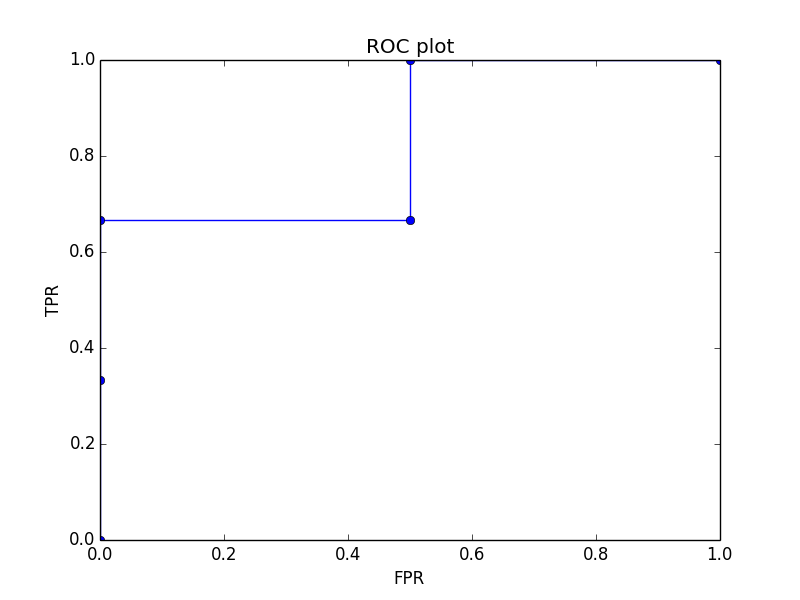
\includegraphics[scale=0.8]{ml1.png}

\end{figure}

$\mbox{AUC}=\frac{5}{6}$, $\ell_{rank}=\frac{1}{6}$. The $\mbox{ROC}$-plot is Figure \ref{pic1}.

\item 
Obviously, $\mbox{AUC} = \text{area of the part below the ROC-curve}$, so it suffices to prove that  $\ell_{rank} = \text{Area } S_{above}$  where $S_{above}\triangleq \text{the part above the }\mbox{ROC} \text{-curve}$.\\
We will prove this by 3 steps. In addition, the Figure \ref{pic2} could be used for illustration of the proof.
\begin{figure}[!bh]\label{pic2}
\caption{Illustration}
\centering
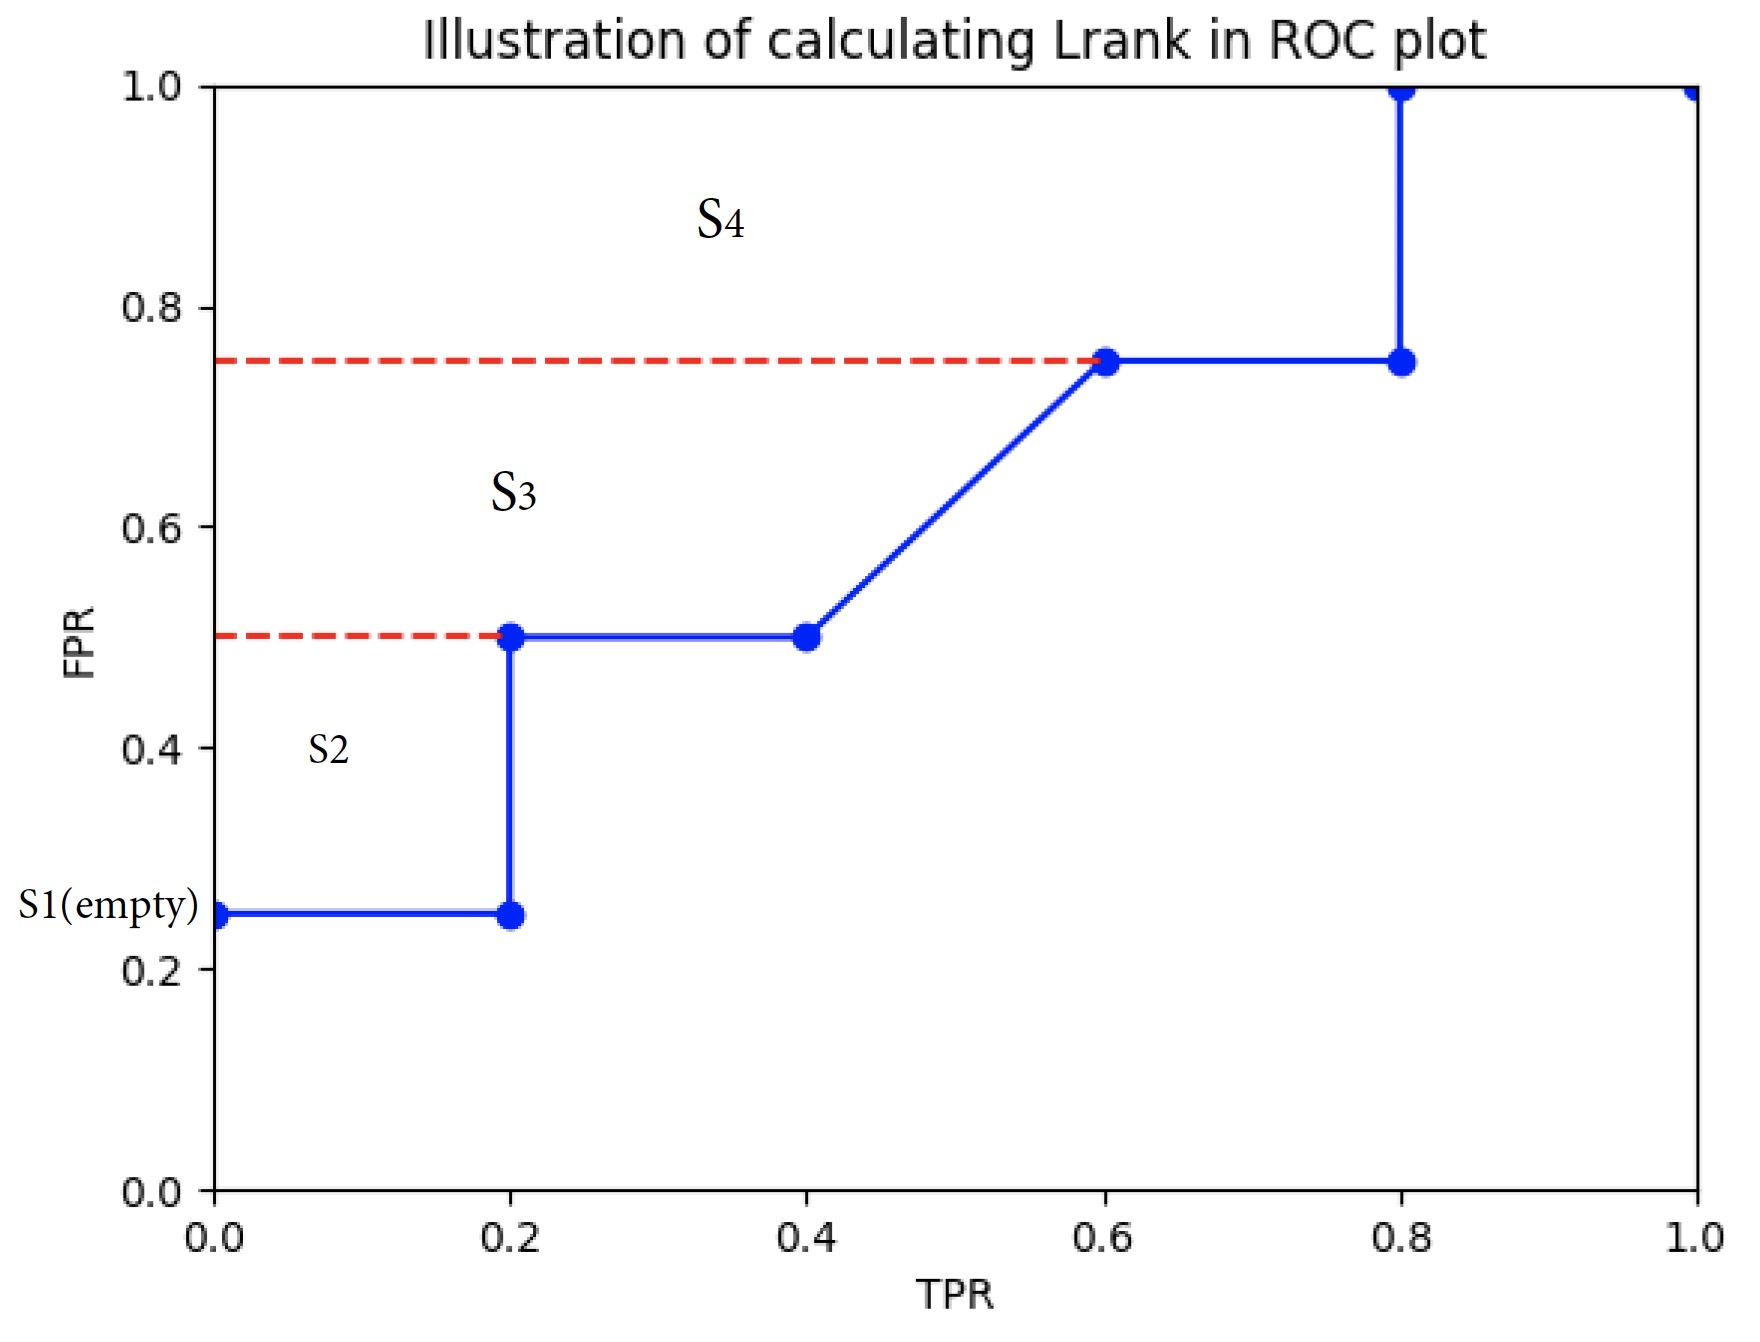
\includegraphics[scale=0.2]{ml2.png}

\end{figure}
\begin{enumerate}[Step 1.]
\item Decomposition of $S_{above}$.

Note that, when plotting $\mbox{AUC}$ curve, for each cut-point-value we are currently considering and given the previous cut point's coordinate $(x,y)$ :

 If there is only one corresponding cut-point in the samples:
 \begin{itemize}
\item if the cut point is true positive, then the previous coordinate will "go up" by $\frac{1}{m^+}$, which results in a new point $(x, y+\frac{1}{m^+})$;
\item  if the cut point is false positive, then the precious coordinate will "go right" by $\frac{1}{m^-}$, which results in a new point $x+\frac{1}{n^-}, y)$
\end{itemize}
Otherwise, there are multiple samples that share the same prediction value. In this case, the new point added will "go up" by $n_1*\frac{1}{m^+}$, and "go right" by $n_2 * \frac{1}{m^-}$, with corresponding coordinate $(x + n_2 * \frac{1}{m^-}, y + n_1*\frac{1}{m^+})$, where $n_1 ( n_2 )$ is the number of positive (negative) samples have  ranked all the same with the current cut-off-value.

We could index the samples in $\mathcal{D^+}$ (the set of positive samples) in decreasing order of prediction values as below shows:
 $$\mathcal{D^+} =\{\mathbf{x}^+_k \mid f(\mathbf{x}^+_k) \geq f(\mathbf{x}^+_{k+1}) \text{ for } k=1,\cdots, m-1, \text{ and } \mathbf{x}^+_k \text{is predicted positive}\}, $$
and let
$$(x^+_k, y^+_k)= \text{ the coordinate of }\mathbf{x}^+_k,$$ 
$$S_k =  \{(x,y) \mid y^+_{k-1} < y\leq y^+_k,0<x<x^+_k \} \quad \quad (\text{set }y^+_0=0).$$  

Therefore,  $S_{above}= \bigcup_{k=1}^{m^+} S_{k}$.

\item Calculation of Area $(S_k)$.

Note that  $\sum_{\mathbf{x}^- \in \mathcal{D}^-} \mathbb{I}(f(\mathbf{x}^+_k)<f(\mathbf{x}^-_k)) + \frac{1}{2}\mathbb{I}(f(\mathbf{x}^+_k)=f(\mathbf{x}^-_k))$ is the number of negative samples ranked before or the same as $\mathbf{x}^+_k$, therefore $x^+_k = \frac{1}{m^-}\sum_{\mathbf{x}^- \in \mathcal{D}^-} \mathbb{I}(f(\mathbf{x}^+_k)<f(\mathbf{x}^-_k)) + \mathbb{I}(f(\mathbf{x}^+_k)=f(\mathbf{x}^-_k))$.


If $\sum_{\mathbf{x}^- \in \mathcal{D}^-} \mathbb{I}(f(\mathbf{x}^+_k)=f(\mathbf{x}^-_k))=0$, which suggests no negative samples are ranked the same as $\mathbf{x}^+_k$, then $S_k$ is a trapezoid; otherwise, it is a rectangle.


In either way,
\begin{equation*}
\text{Area }( S_k) = \frac{1}{m^+} \frac{1}{m^-}\sum_{\mathbf{x}^- \in \mathcal{D}^-} (\mathbb{I}(f(\mathbf{x}^+_k)<f(\mathbf{x}^-_k)) +\frac{1}{2} \mathbb{I}(f(\mathbf{x}^+_k)=f(\mathbf{x}^-_k)).
\end{equation*}

\item Calculaiton of Area $(S_{above})$.

Since  $\{S_k\}_{k=1}^{m^+}$ are mutually disjoint,
\begin{equation*}
\begin{split}
\text{Area } (S_{above}) &= \bigcup_{k=1}^m \text{Area }(S_{k})
\\
&= \sum_{k=1}^{m^+}\frac{1}{m^+} \frac{1}{m^-}\sum_{\mathbf{x}^- \in \mathcal{D}^-}  (\mathbb{I}(f(\mathbf{x}^+_k)<f(\mathbf{x}^-_k)) +\frac{1}{2} \mathbb{I}(f(\mathbf{x}^+_k)=f(\mathbf{x}^-_k))
\\
&= \frac{1}{m^+} \frac{1}{m^-}\sum_{\mathbf{x}^+ \in \mathcal{D}^+}\sum_{\mathbf{x}^- \in \mathcal{D}^-} (\mathbb{I}(f(\mathbf{x}^+_k)<f(\mathbf{x}^-_k)) +\frac{1}{2} \mathbb{I}(f(\mathbf{x}^+_k)=f(\mathbf{x}^-_k))
\\
&=\ell_{rank}.
\end{split}
\end{equation*}
\end{enumerate}
\qed




\end{enumerate}
\end{mySol}

\newpage
\section{[附加题10pts] Expected Prediction Error}
对于最小二乘线性回归问题,我们假设其线性模型为:
\begin{equation}
	y=\textbf{x}^T  \bm{ \beta } + \epsilon , 
\end{equation}
其中$\epsilon$为噪声满足$\epsilon\sim N(0,\sigma^2)$。我们记训练集$\mathcal{D}$中的样本特征为$\textbf{X}\in \mathbb{R}^{p \times n}$,标记为$\textbf{Y}\in \mathbb{R}^{n}$,其中$n$为样本数,$p$为特征维度。
已知线性模型参数的估计为:
\begin{equation}
	\hat{\bm{\beta}}=(\textbf{X}\textbf{X}^T)^{-1}\textbf{X}\textbf{Y}.	
\end{equation}

对于给定的测试样本$\textbf{x}_0$,记$\mathbf{EPE}(\textbf{x}_0)$为其预测误差的期望 (Expected Predication Error),试证明,
\[
	\mathbf{EPE}(\textbf{x}_0) = \sigma^2+\mathbb{E}_{\mathcal{D}}[\textbf{x}_0^T(\textbf{X}\textbf{X}^T)^{-1}\textbf{x}_0\sigma^2].
\]

要求证明中给出详细的步骤与证明细节。(提示:$\mathbf{EPE}(\textbf{x}_0)=\mathbb{E}_{y_0|\textbf{x}_0} \mathbb{E}_{\mathcal{D}}[(y_0-\hat{y}_0)^2]$,可以参考书中第45页关于方差-偏差分解的证明过程。)

\begin{myProof}
We will give a proof by three steps.
\begin{enumerate}[Step 1.]
\item Preparation

First, we need to clarify some notations.
\begin{itemize}
\item
$\hat{\bm{\beta}}$ is the least-square-estimate coefficient, with
\begin{equation*}
\hat{\bm{\beta}} = (\textbf{X}\textbf{X}^T)^{-1}\textbf{X}\textbf{Y} = (\textbf{X}\textbf{X}^T)^{-1}\textbf{X}(\textbf{X}^T \bm{\beta} +\epsilon) = \bm{\beta} + (\textbf{X}\textbf{X}^T)^{-1}X\epsilon.
\end{equation*}
$\hat{\bm{\beta}}$ is an unbiased estimator of $\bm{\beta}$ since
\begin{equation*}
\mathbb{E} [\hat{\bm{\beta}}]=\mathbb{E} [ \bm{\beta} + (\textbf{X}\textbf{X}^T)^{-1}\textbf{X}\epsilon] = \bm{\beta}.
\end{equation*}
\item 
$y_0$ is the observation value, with
\begin{equation} \label{y0}
y_0 = \textbf{x}_0^T \beta +\epsilon.
\end{equation}
\item
$\hat{y}_0$ is the prediction value, with
\begin{equation} \label{yhat0}
\hat{y}_0 = \textbf{x}_0^T \hat{\beta} = \textbf{x}_o^T \bm{\beta} + \textbf{x}_0^T (\textbf{X}\textbf{X}^T)^{-1} \textbf{X} \epsilon .
\end{equation}

\item Define the expected prediction value $\bar{y}_0$ with 
\begin{equation} \label{def_ybar0}
\bar{y}_0 \triangleq \mathbb{E}_{\mathcal{D}} [\hat{y}_0].
\end{equation}
Then substituting (\ref{yhat0}) into (\ref{def_ybar0}), we obtain
\begin{equation} \label{ybar0}
\bar{y}_0 = \mathbb{E}_{\mathcal{D}}[ \textbf{x}_o^T \bm{\beta} + \textbf{x}_0^T (\textbf{X}\textbf{X}^T)^{-1} \textbf{X} \epsilon] =   \textbf{x}_o^T \bm{\beta} + \textbf{x}_0^T (\textbf{X}\textbf{X}^T)^{-1} \textbf{X} \epsilon.
\end{equation}

\end{itemize}

\item Decomposition of $\mathbf{EPE}(\textbf{x}_0)$ 

\begin{equation}\label{EPE}
\begin{split}
\mathbf{EPE}(\textbf{x}_0)&=\mathbb{E}_{y_0|\textbf{x}_0} \mathbb{E}_{\mathcal{D}}[(y_0-\hat{y}_0)^2  \\
&=\mathbb{E}_{y_0|\textbf{x}_0} \mathbb{E}_{\mathcal{D}}[(y_0-\bar{y}_0 + \bar{y}_0- \hat{y}_0)^2  \\
&= \mathbb{E}_{y_0|\textbf{x}_0} \mathbb{E}_{\mathcal{D}}[(y_0-\bar{y}_0)^2 + \mathbb{E}_{y_0|\textbf{x}_0} \mathbb{E}_{\mathcal{D}}[(\bar{y}_0-\hat{y}_0)^2 + 2 \mathbb{E}_{y_0|\textbf{x}_0} \mathbb{E}_{\mathcal{D}}[(y_0-\bar{y}_0)(\bar{y}_0 - \hat{y}_0)
\end{split}
\end{equation}

\begin{itemize}
\item The first item

Using (\ref{y0} and (\ref{ybar0}), we have 
\begin{equation}\label{first-item}
\begin{split}
\mathbb{E}_{y_0|\textbf{x}_0} \mathbb{E}_{\mathcal{D}}[(y_0-\bar{y}_0)^2 &= \mathbb{E}_{y_0|\textbf{x}_0} \mathbb{E}_{\mathcal{D}}[(\textbf{x}_0^T \bm{\beta} + \epsilon - \textbf{x}_0^T \bm{\beta})^2]\\
&= \mathbb{E}_{y_0|\textbf{x}_0} \mathbb{E}_{\mathcal{D}} [\epsilon ^2]\\
&=\sigma ^2
\end{split}
\end{equation}

\item The second item

Using (\ref{ybar0}) and (\ref{yhat0}), we have
\begin{equation*}
\begin{split}
\mathbb{E}_{y_0|\textbf{x}_0} \mathbb{E}_{\mathcal{D}}[(\bar{y}_0-\hat{y}_0)^2 ]
&= \mathbb{E}_{y_0|\textbf{x}_0} \mathbb{E}_{\mathcal{D}}[(\textbf{x}_0^T \bm{\beta} - \textbf{x}_0^T\bm{\beta} + \textbf{x}_0^T(\textbf{X}\textbf{X}^T)^{-1} \textbf{X} \epsilon)^2] \\
&= \mathbb{E}_{y_0|\textbf{x}_0} \mathbb{E}_{\mathcal{D}}[(\textbf{x}_0^T(\textbf{X}\textbf{X}^T)^{-1} \textbf{X} \epsilon)^2 ]\\
&= \mathbb{E}_{y_0|\textbf{x}_0} \mathbb{E}_{\mathcal{D}}[(\textbf{x}_0^T(\textbf{X}\textbf{X}^T)^{-1} \textbf{X} \epsilon)(\textbf{x}_0^T(\textbf{X}\textbf{X}^T)^{-1} \textbf{X} \epsilon)] \\
&= \mathbb{E}_{y_0|\textbf{x}_0} \mathbb{E}_{\mathcal{D}}[(\textbf{x}_0^T(\textbf{X}\textbf{X}^T)^{-1} \textbf{X}) (\textbf{x}_0^T(\textbf{X}\textbf{X}^T)^{-1} \textbf{X})\epsilon ^2] 
\end{split}
\end{equation*}
Since $\textbf{X}\textbf{X}^T$ is symmetric, which suggests $\textbf{x}_0^T(\textbf{X}\textbf{X}^T)^{-1} \textbf{X}$ is a quadratic form, we have
$$\textbf{x}_0^T(\textbf{X}\textbf{X}^T)^{-1} \textbf{X} = \textbf{X}^T(\textbf{X}\textbf{X}^T)^{-1} \textbf{x}_0$$. Therefore,
\begin{equation}\label{second-item}
\begin{split}
\mathbb{E}_{y_0|\textbf{x}_0} \mathbb{E}_{\mathcal{D}}[(\bar{y}_0-\hat{y}_0)^2 ] 
&= \mathbb{E}_{y_0|\textbf{x}_0} \mathbb{E}_{\mathcal{D}}[(\textbf{x}_0^T(\textbf{X}\textbf{X}^T)^{-1} \textbf{X}) (\textbf{X}^T(\textbf{X}\textbf{X}^T)^{-1} \textbf{x}_0)\epsilon ^2] \\
&= \mathbb{E}_{y_0|\textbf{x}_0} \mathbb{E}_{\mathcal{D}}[\textbf{x}_0^T(\textbf{X}\textbf{X}^T)^{-1} (\textbf{X} \textbf{X}^T) (\textbf{X}\textbf{X}^T)^{-1} \textbf{x}_0 \epsilon ^2]  \\
&= \mathbb{E}_{\mathcal{D}}[\textbf{x}_0^T(\textbf{X}\textbf{X}^T)^{-1} \textbf{x}_0\sigma ^2] 
\end{split}
\end{equation}

\item The third item
Because of the definition of $\hat{y}_0$  (\ref{def_ybar0}), 
 \begin{equation}\label{third-item}
 {E}_{\mathcal{D}}[(y_0-\bar{y}_0)(\bar{y}_0 - \hat{y}_0) = 0.
 \end{equation}
 
\end{itemize}

\item Putting together

Substituting (\ref{first-item}), \ref{second-item}) and (\ref{third-item}) into (\ref{EPE}), we obtain the desired simplified decomposition of $\mathbf{EPE}(\textbf{x}_0)$.
\end{enumerate}
\qed
\end{myProof}




\end{document}